\section{Implementation}

\subsection{User interface}

\subsubsection{New project page}
Form interface allowing users to create a new LaTeX project, with options to set project name, template selection, and initial configuration, as seen in Figure \ref{fig:ui-newproject}.

\begin{figure}[htb]
    \centering
    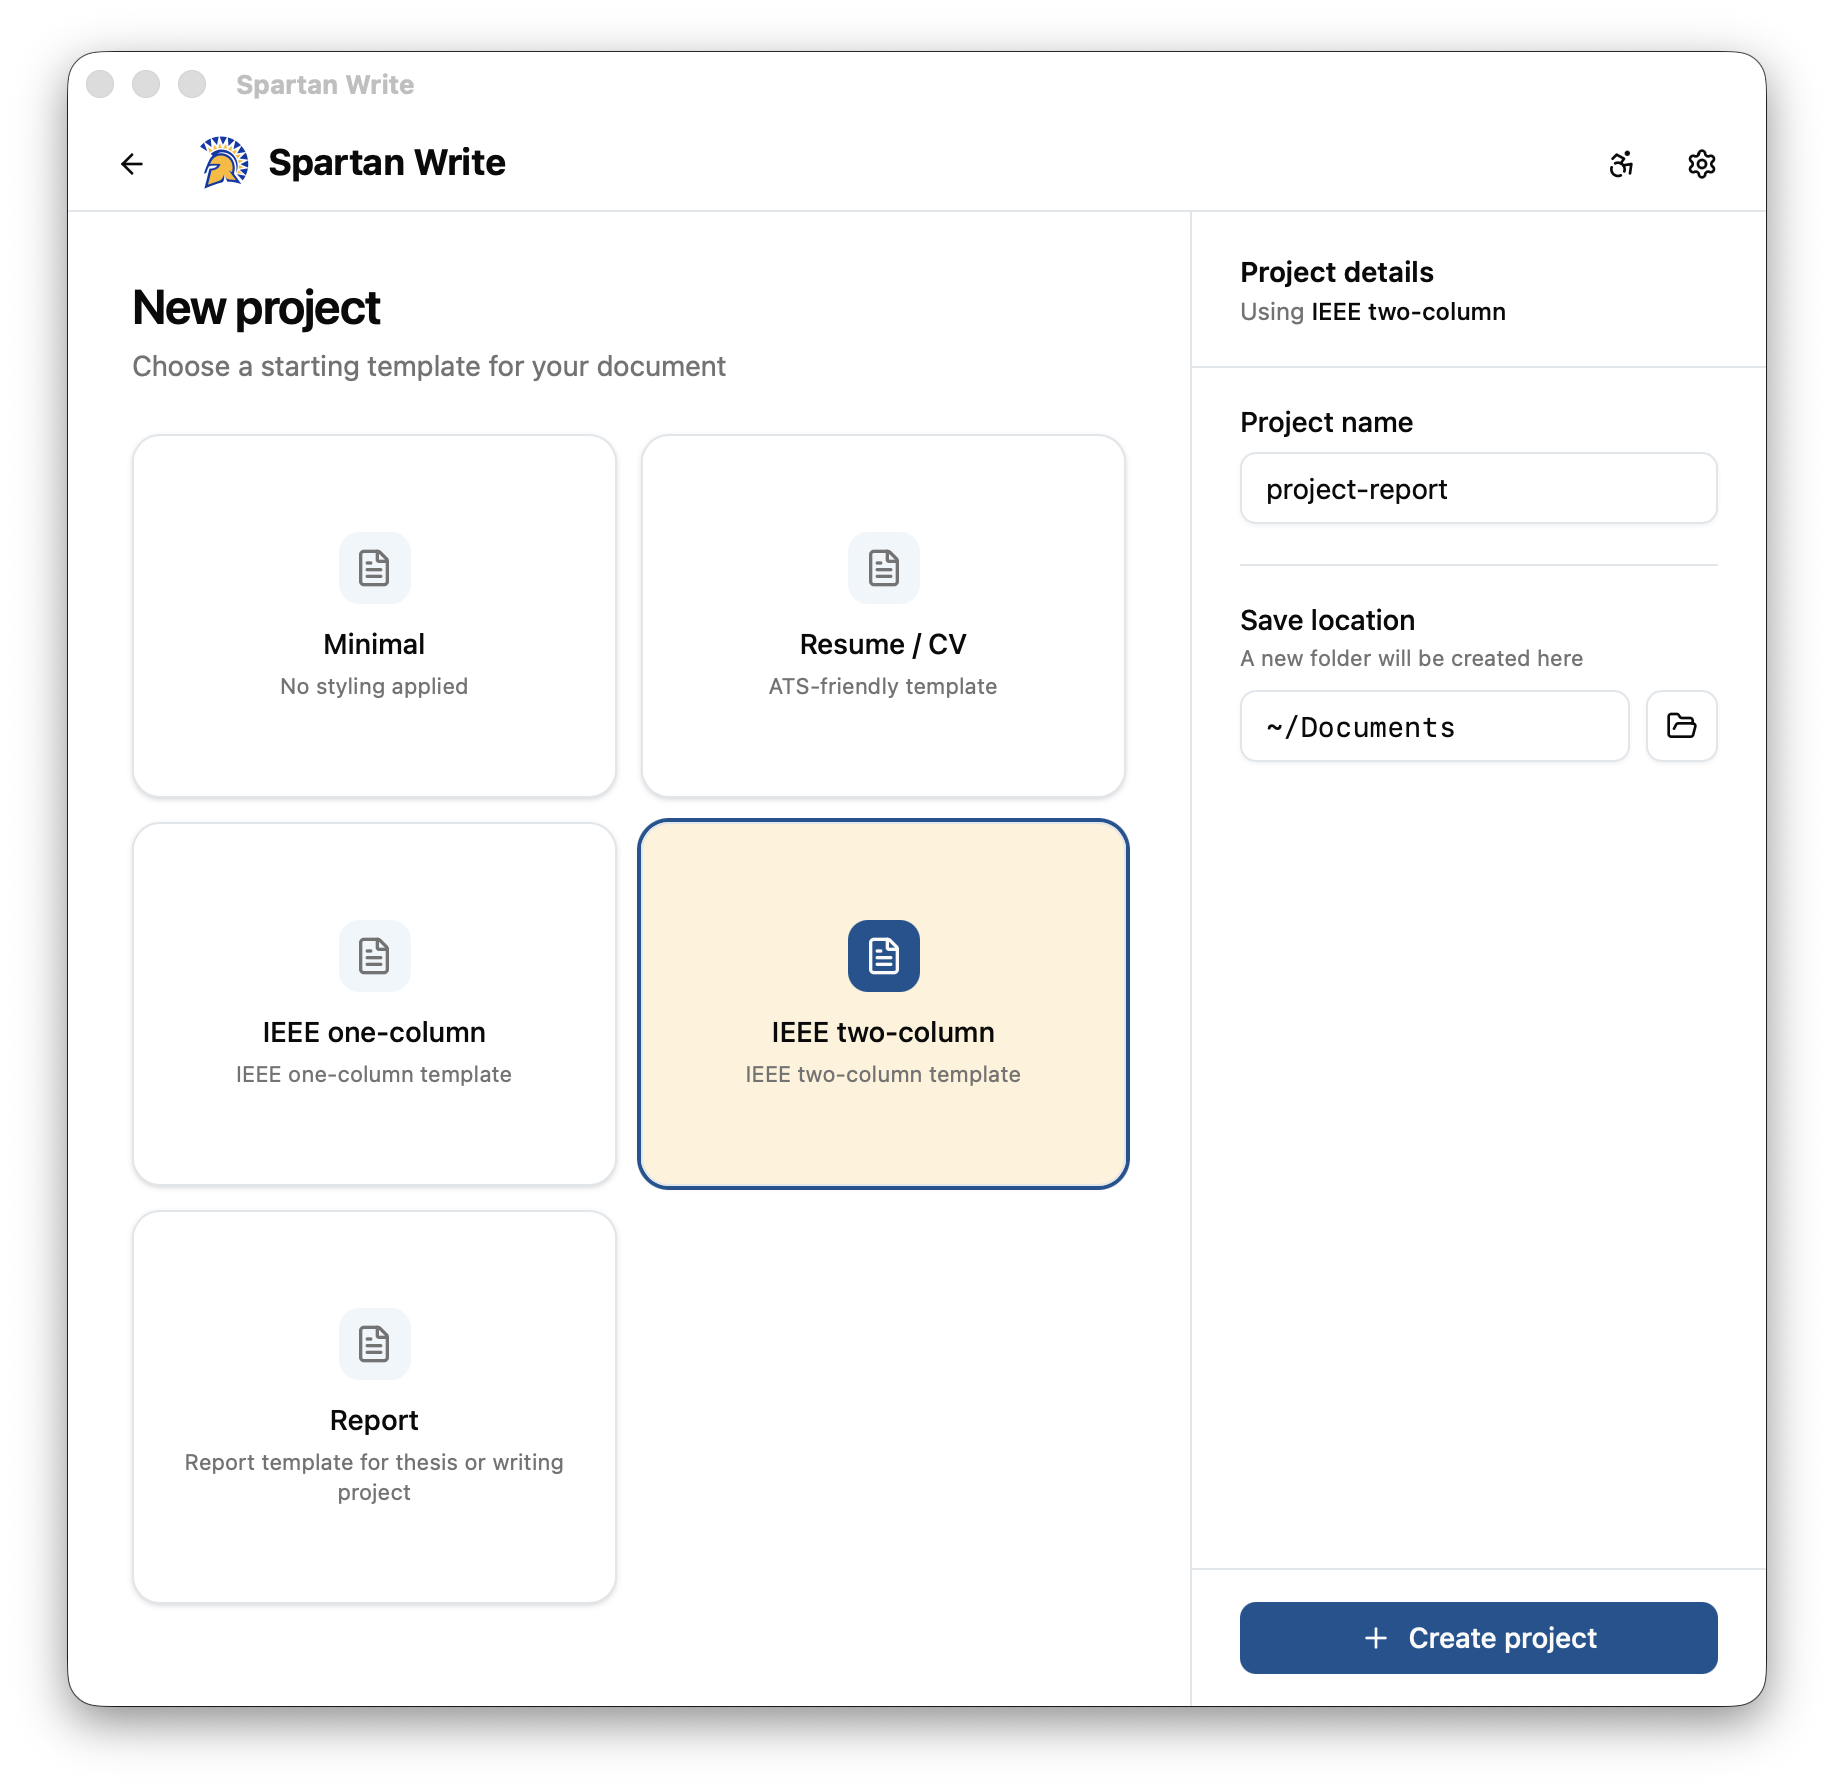
\includegraphics[width=0.67\linewidth]{figures/ui-newproject.png}
    \caption{New project template selection interface}
    \label{fig:ui-newproject}
\end{figure}

\subsubsection{Recent projects page}
Dashboard displaying a list of the user's recently accessed projects with options to open, rename, or delete them, as seen in Figure \ref{fig:ui-dashboard}.

\begin{figure}[htb]
    \centering
    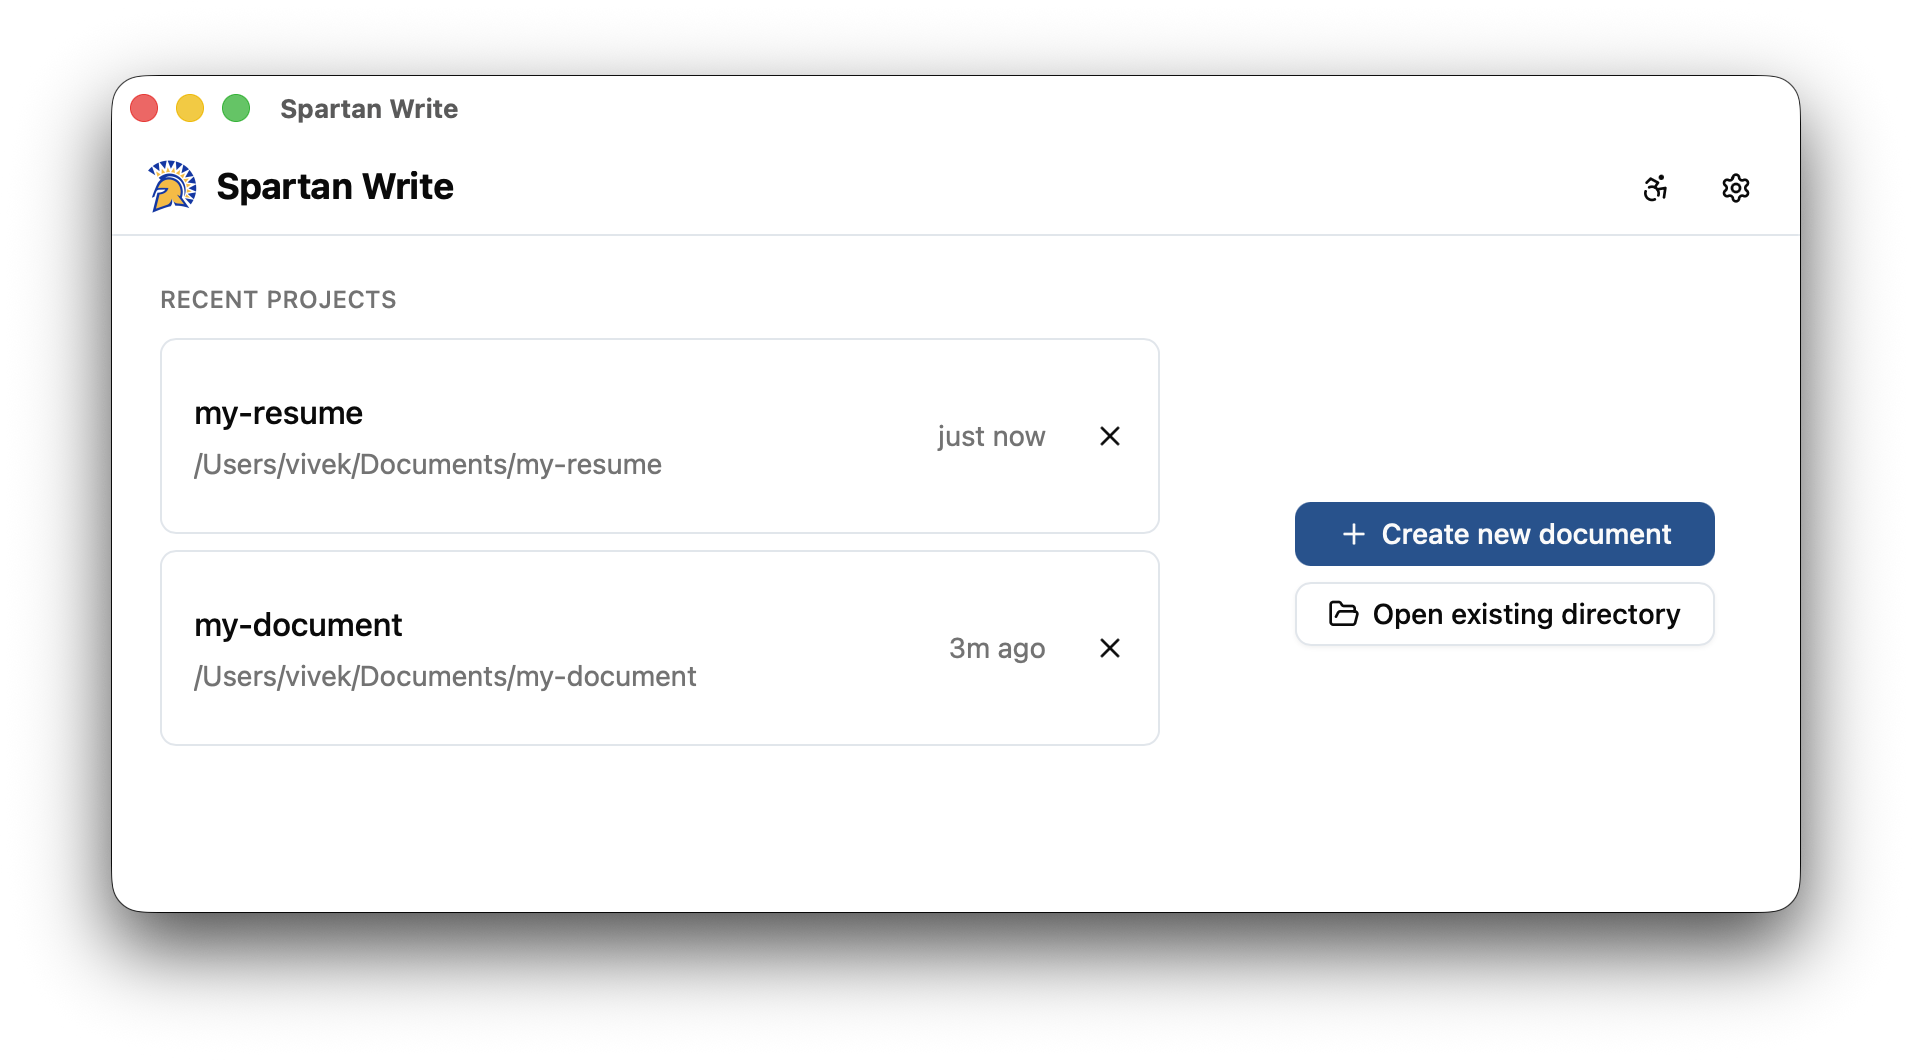
\includegraphics[width=0.67\linewidth]{figures/ui-dashboard.png}
    \caption{Dashboard interface showing recent projects}
    \label{fig:ui-dashboard}
\end{figure}

\subsubsection{Project preview}
The project workspace with the preview interface. The user can see their document draft and interact with a chatbot using the conversation panel, as seen in Figure \ref{fig:ui-docpreview}.

\begin{figure}[htb]
    \centering
    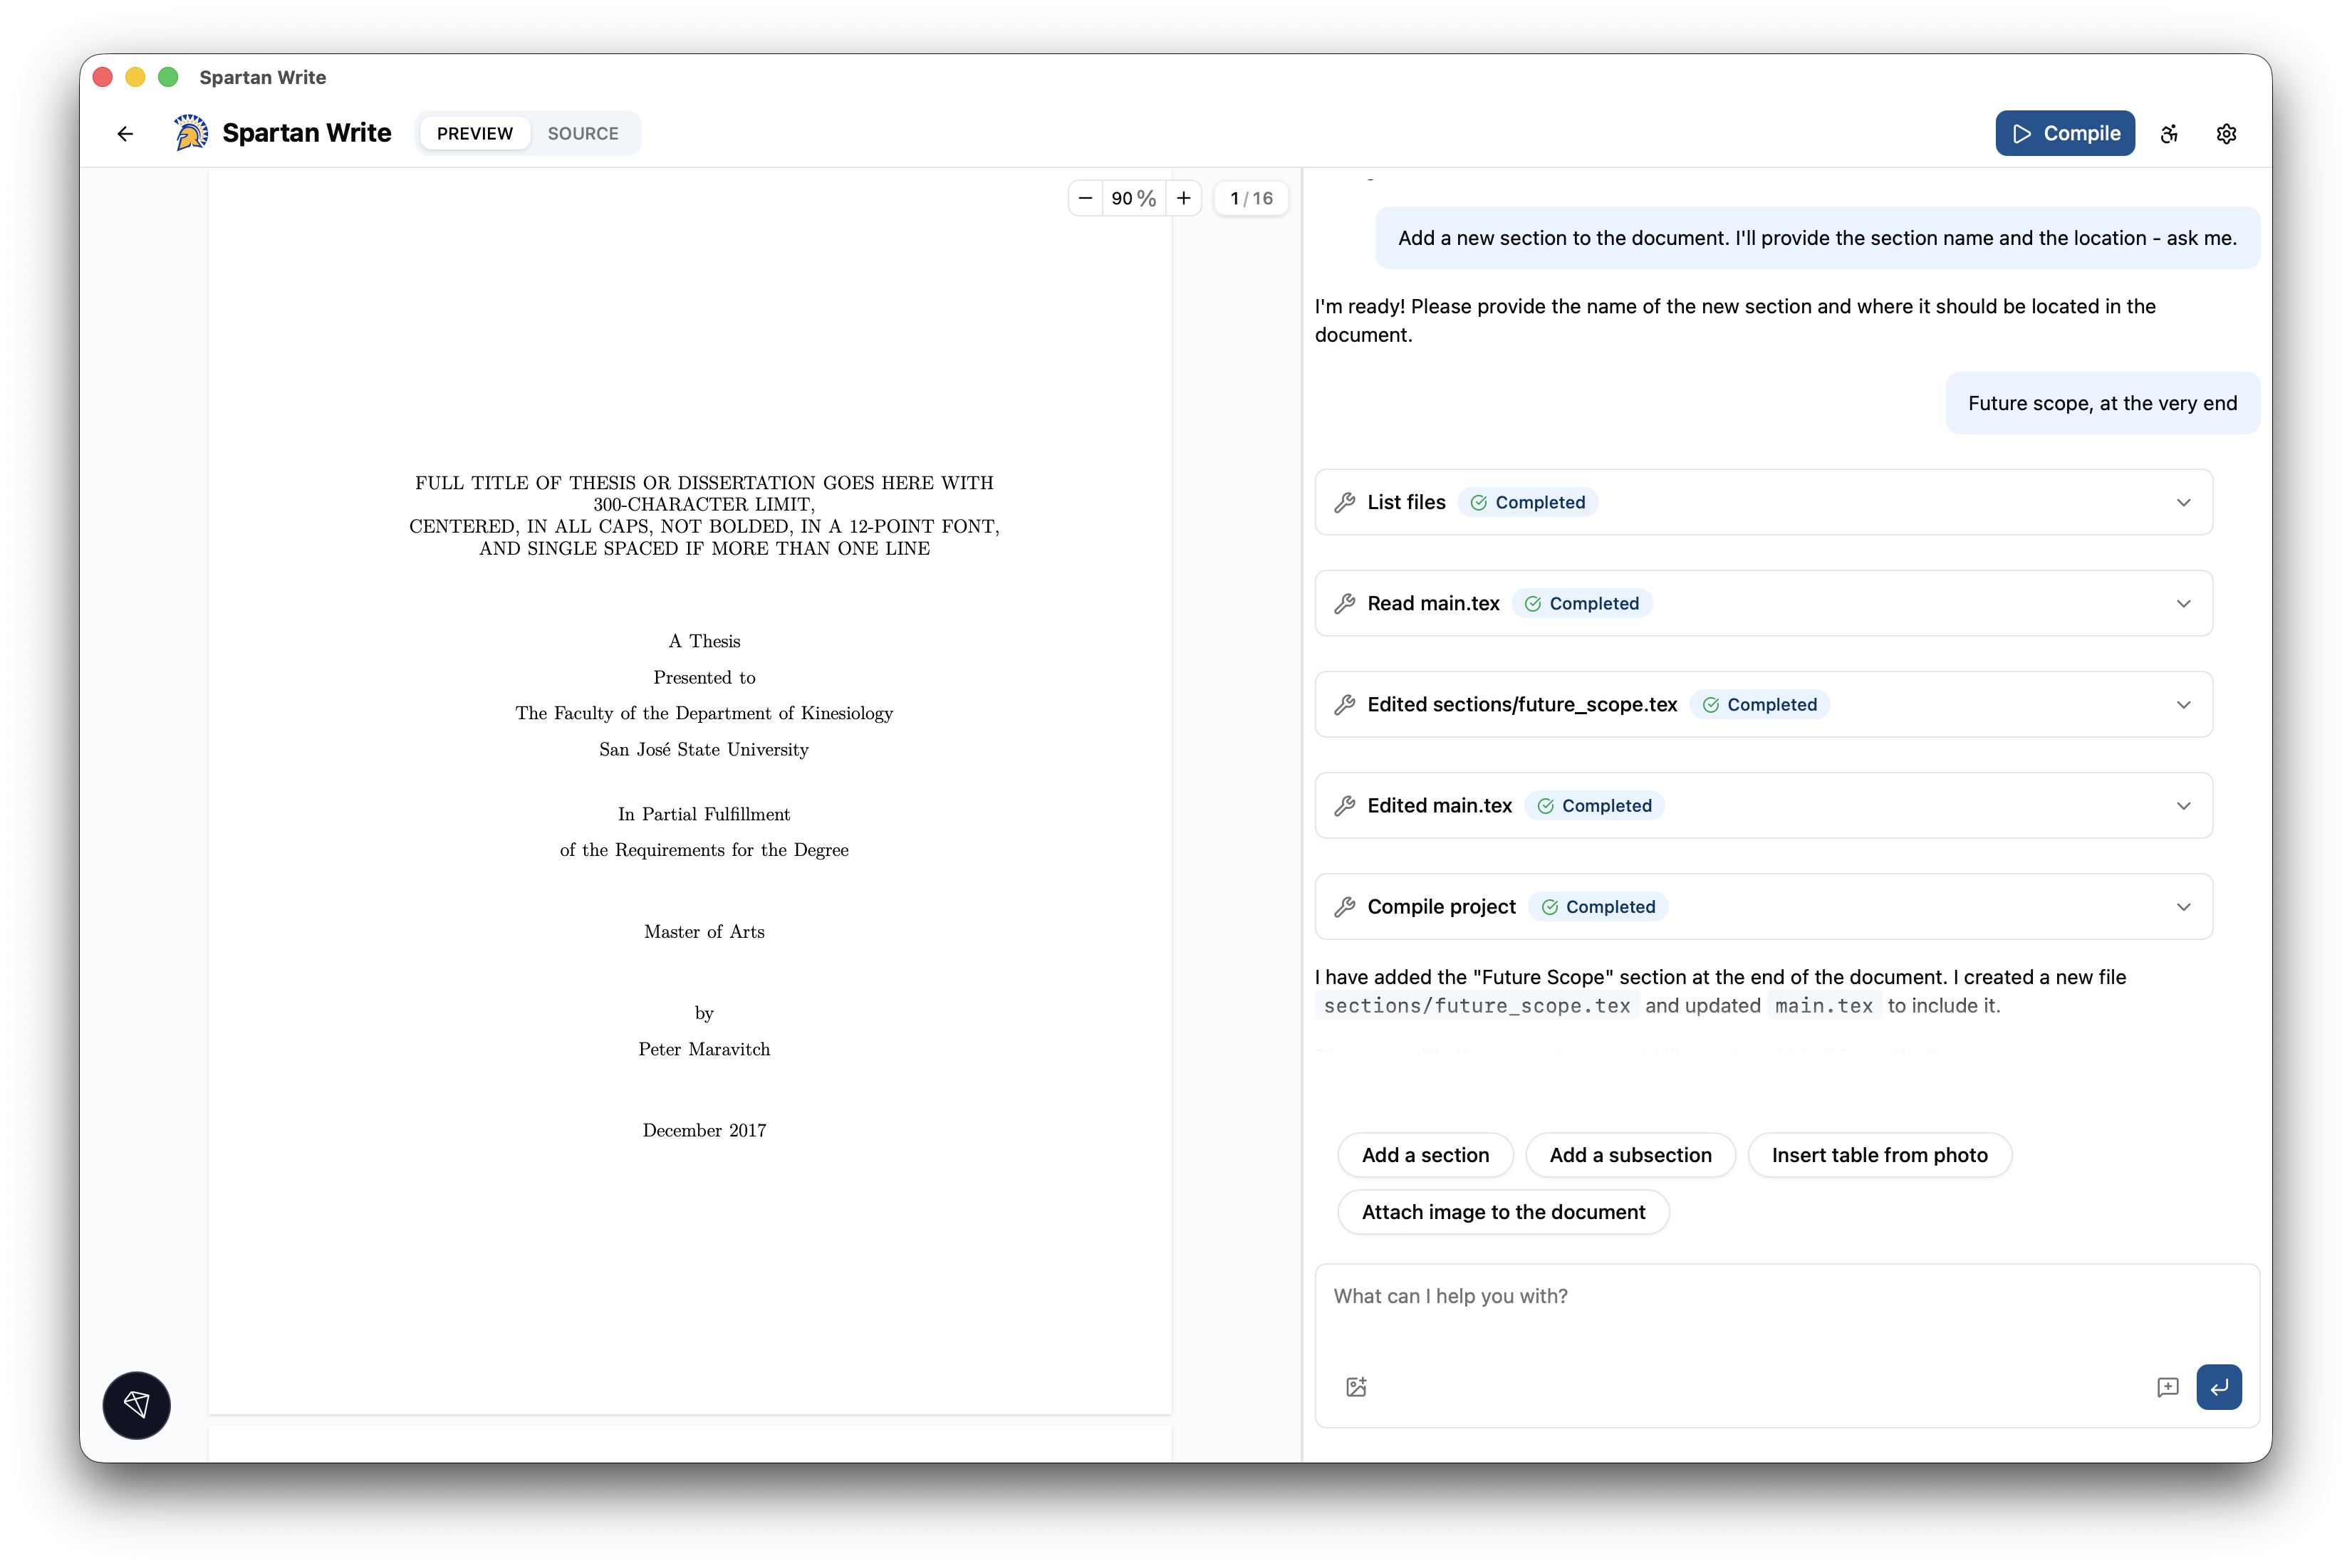
\includegraphics[width=\linewidth]{figures/ui-docpreview.png}
    \caption{Live PDF preview provides immediate feedback alongside conversational editing.}
    \label{fig:ui-docpreview}
\end{figure}

\subsubsection{Source editor}
Text editor for directly editing \LaTeX\ source code with syntax highlighting, line numbers, and code assistance features, as seen in Figure \ref{fig:ui-editor}.

\begin{figure}[htb]
    \centering
    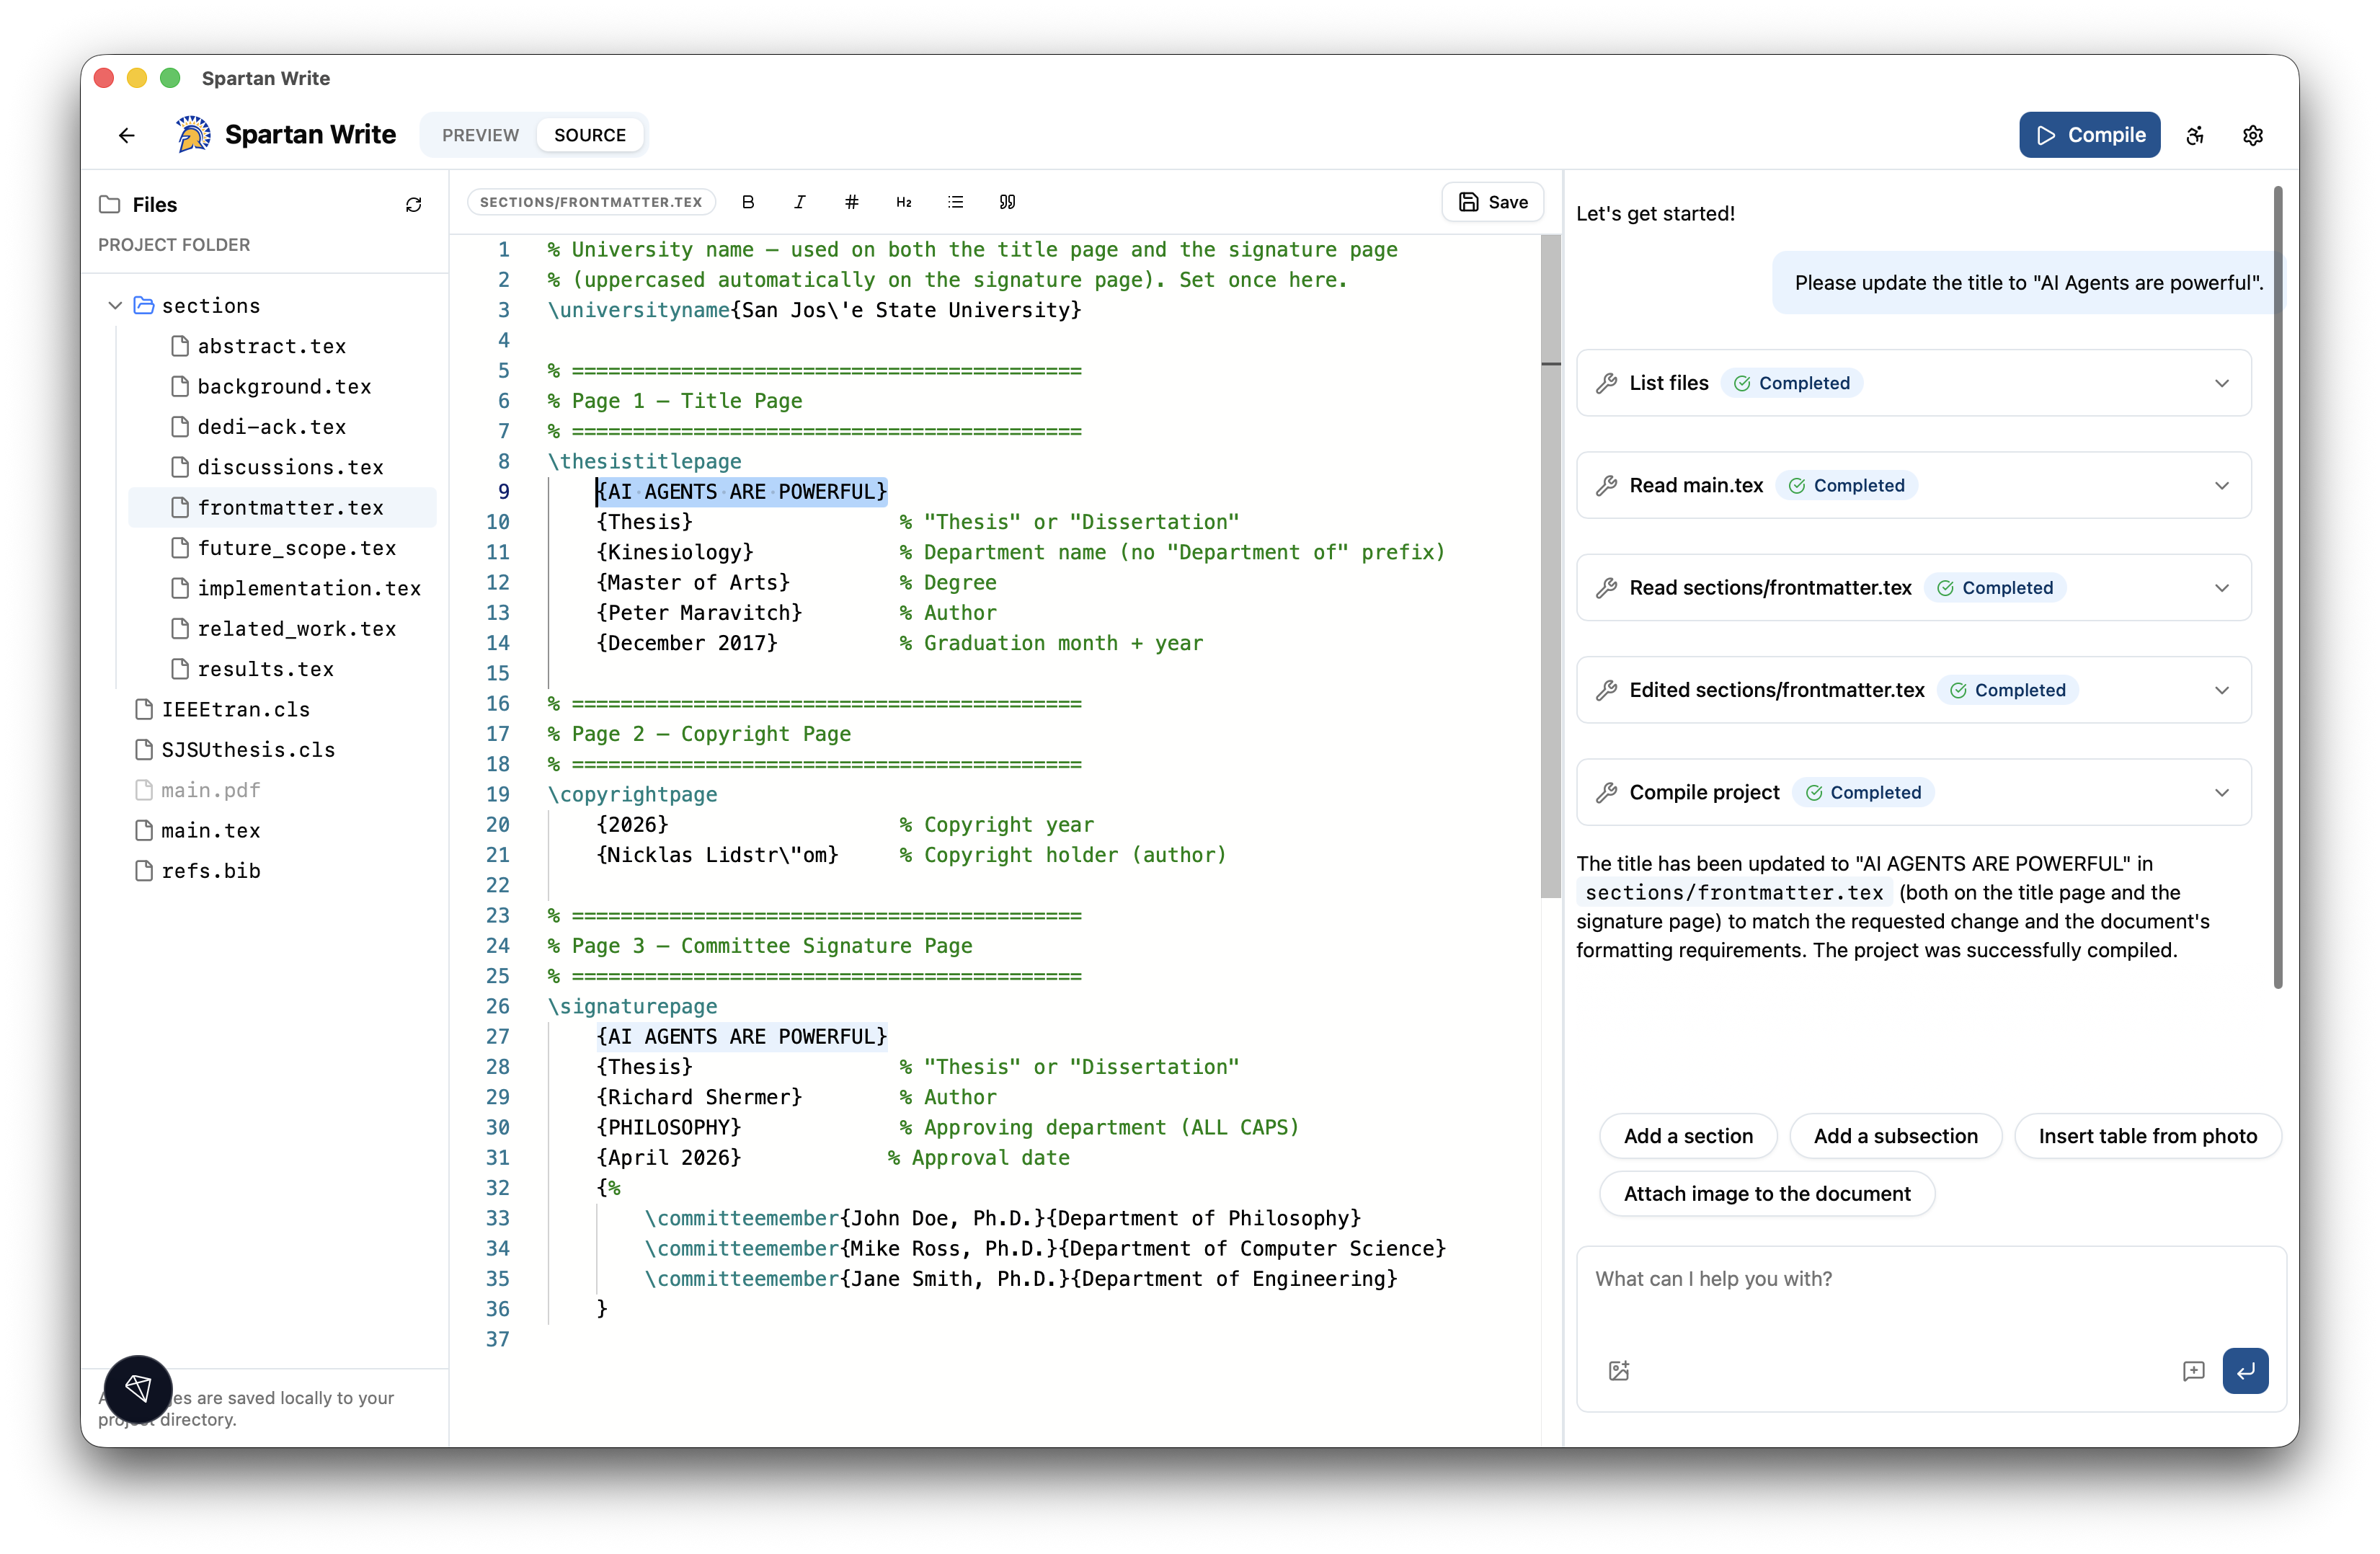
\includegraphics[width=\linewidth]{figures/ui-editor.png}
    \caption{Syntax-highlighted source editor preserves power-user control for direct edits.}
    \label{fig:ui-editor}
\end{figure}

\subsection{Build pipeline}

The build pipeline consists of several stages, as each component of the application needs to be compiled and packaged.

\begin{enumerate}
    \item First, the sidecar is compiled and packaged into a standalone binary using the PyInstaller system.
    \item The Tectonic binary for LaTeX compilation is then downloaded from its repository.
    \item Both of these binaries are copied into the Tauri source code and registered to be bundled.
    \item The Tauri frontend is then compiled. This includes the other binaries and creates an installable package.
    \item These steps are repeated on Windows, MacOS, and Ubuntu systems, in order to generate installable packages for each OS.
    \item In parallel to this, the server is built and packaged as a Docker image, ready to be pulled and deployed on a server.
\end{enumerate}

\subsection{Agent design}

\subsubsection{System prompt}

The agent operates under a comprehensive system prompt that defines its role as a \LaTeX\ assistant capable of understanding user requests and making intelligent document modifications.
The prompt establishes clear guidelines for workflow (list files $\rightarrow$ read $\rightarrow$ edit $\rightarrow$ compile), file organization conventions, and safety principles (minimal changes, user-provided content only, no unsolicited additions).
This prompt-based design ensures consistent, predictable behavior aligned with document integrity best practices.
The complete system prompt can be found in Appendix \ref{apx:system-prompt}.

\subsubsection{Architecture}

The agent is implemented as a LangGraph state machine with a deterministic execution graph \cite{langgraph}.
It maintains state across multi-turn conversations, enabling the agent to reference prior context, track intermediate results, and make cumulative edits across multiple user interactions.
The graph structure ensures reliable state transitions and supports checkpoint-based persistence for conversation recovery.

\subsubsection{Tool suite}

The agent has access to seven core tools, as tabulated in Table \ref{tab:agent_tools}.

\begin{table}[htbp]
\centering
\begin{tabular}{|l|p{8cm}|}
\hline
\textbf{Tool name} & \textbf{Description} \\
\hline
\texttt{read\_file\_tool} & Read the contents of any file in the project directory \\
\hline
\texttt{edit\_file\_tool} & Create new files or modify existing files with complete content \\
\hline
\texttt{delete\_file\_tool} & Remove files from the project directory \\
\hline
\texttt{rename\_file\_tool} & Rename or move files within the project, updating all references \\
\hline
\texttt{list\_files\_tool} & Browse and list the project structure recursively or non-recursively \\
\hline
\texttt{compile\_latex\_tool} & Invoke LaTeX compilation and return status and error messages \\
\hline
\texttt{load\_attached\_image\_tool} & Manage image workflows by moving attached images into the figures directory \\
\hline
\end{tabular}
\caption{Tools available to the agent}
\label{tab:agent_tools}
\end{table}

\subsubsection{Tool invocation flow}

When the agent decides to take an action, it invokes the appropriate tool and receives structured output (success/failure, file paths, error messages).
Tool results are fed back into the agent loop, allowing it to respond to outcomes, handle errors, or request clarification from the user.
This interactive loop enables iterative refinement and recovery from failures.

A typical user request is handled as follows.

\begin{enumerate}
    \item The agent reads the user request and starts by using the list\_files\_tool to understand the directory structure.
    \item Then it reads main.tex, as it indicates the layout of each section.
    \item Based on the user's request, the agent then reads the specific section or sections needed to solve the problem.
    \item If there is an image, the agent uses the appropriate tool to import the image into the project.
    \item The agent writes to the desired files as requested by the user.
    \item The compilation tool is then invoked to check for errors. In case of any errors, the agent repeats the process to fix the error.
    \item Finally, the agent responds with a summary of its actions.
\end{enumerate}

A sample run is depicted in Figure \ref{fig:agent-convo}.

\begin{figure}[htbp]
    \centering
    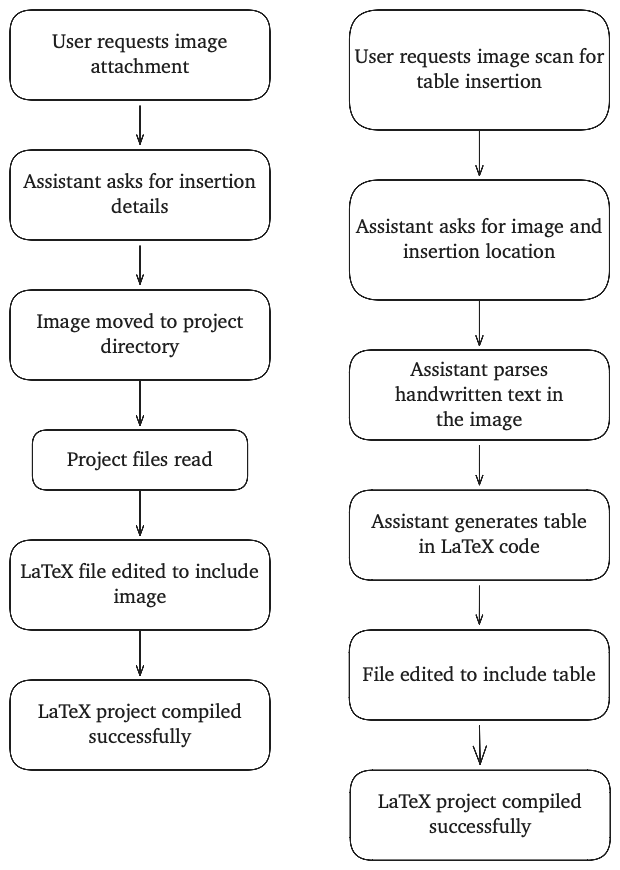
\includegraphics[width=0.9\linewidth]{figures/agent-convo.excalidraw.png}
    \caption{Agent maintains context across multi-turn conversations for iterative refinement.}
    \label{fig:agent-convo}
\end{figure}

\subsubsection{Token usage metrics}

Every agent interaction is tracked and transmitted to PostHog \cite{posthog} to capture comprehensive performance data.
This includes precise token consumption, measuring both input and output volume, tagged with structured metadata such as user ID, model specifications, tool invocations, and session outcomes.
By aggregating these metrics by user, model, and time period, the system provides granular insights into computational costs and infrastructure scaling.
These data points power real-time dashboards that monitor LLM quality and user feedback, directly informing decisions regarding billing logic, usage quotas, and feature development.

The dashboard is seen in Figure \ref{fig:posthog-dashboard}, providing a high level visual overview of the usage, performance, and cost analysis of the application, while Figure \ref{fig:posthog-userwise} shows the usage per user.

\begin{figure}[htb]
    \centering
    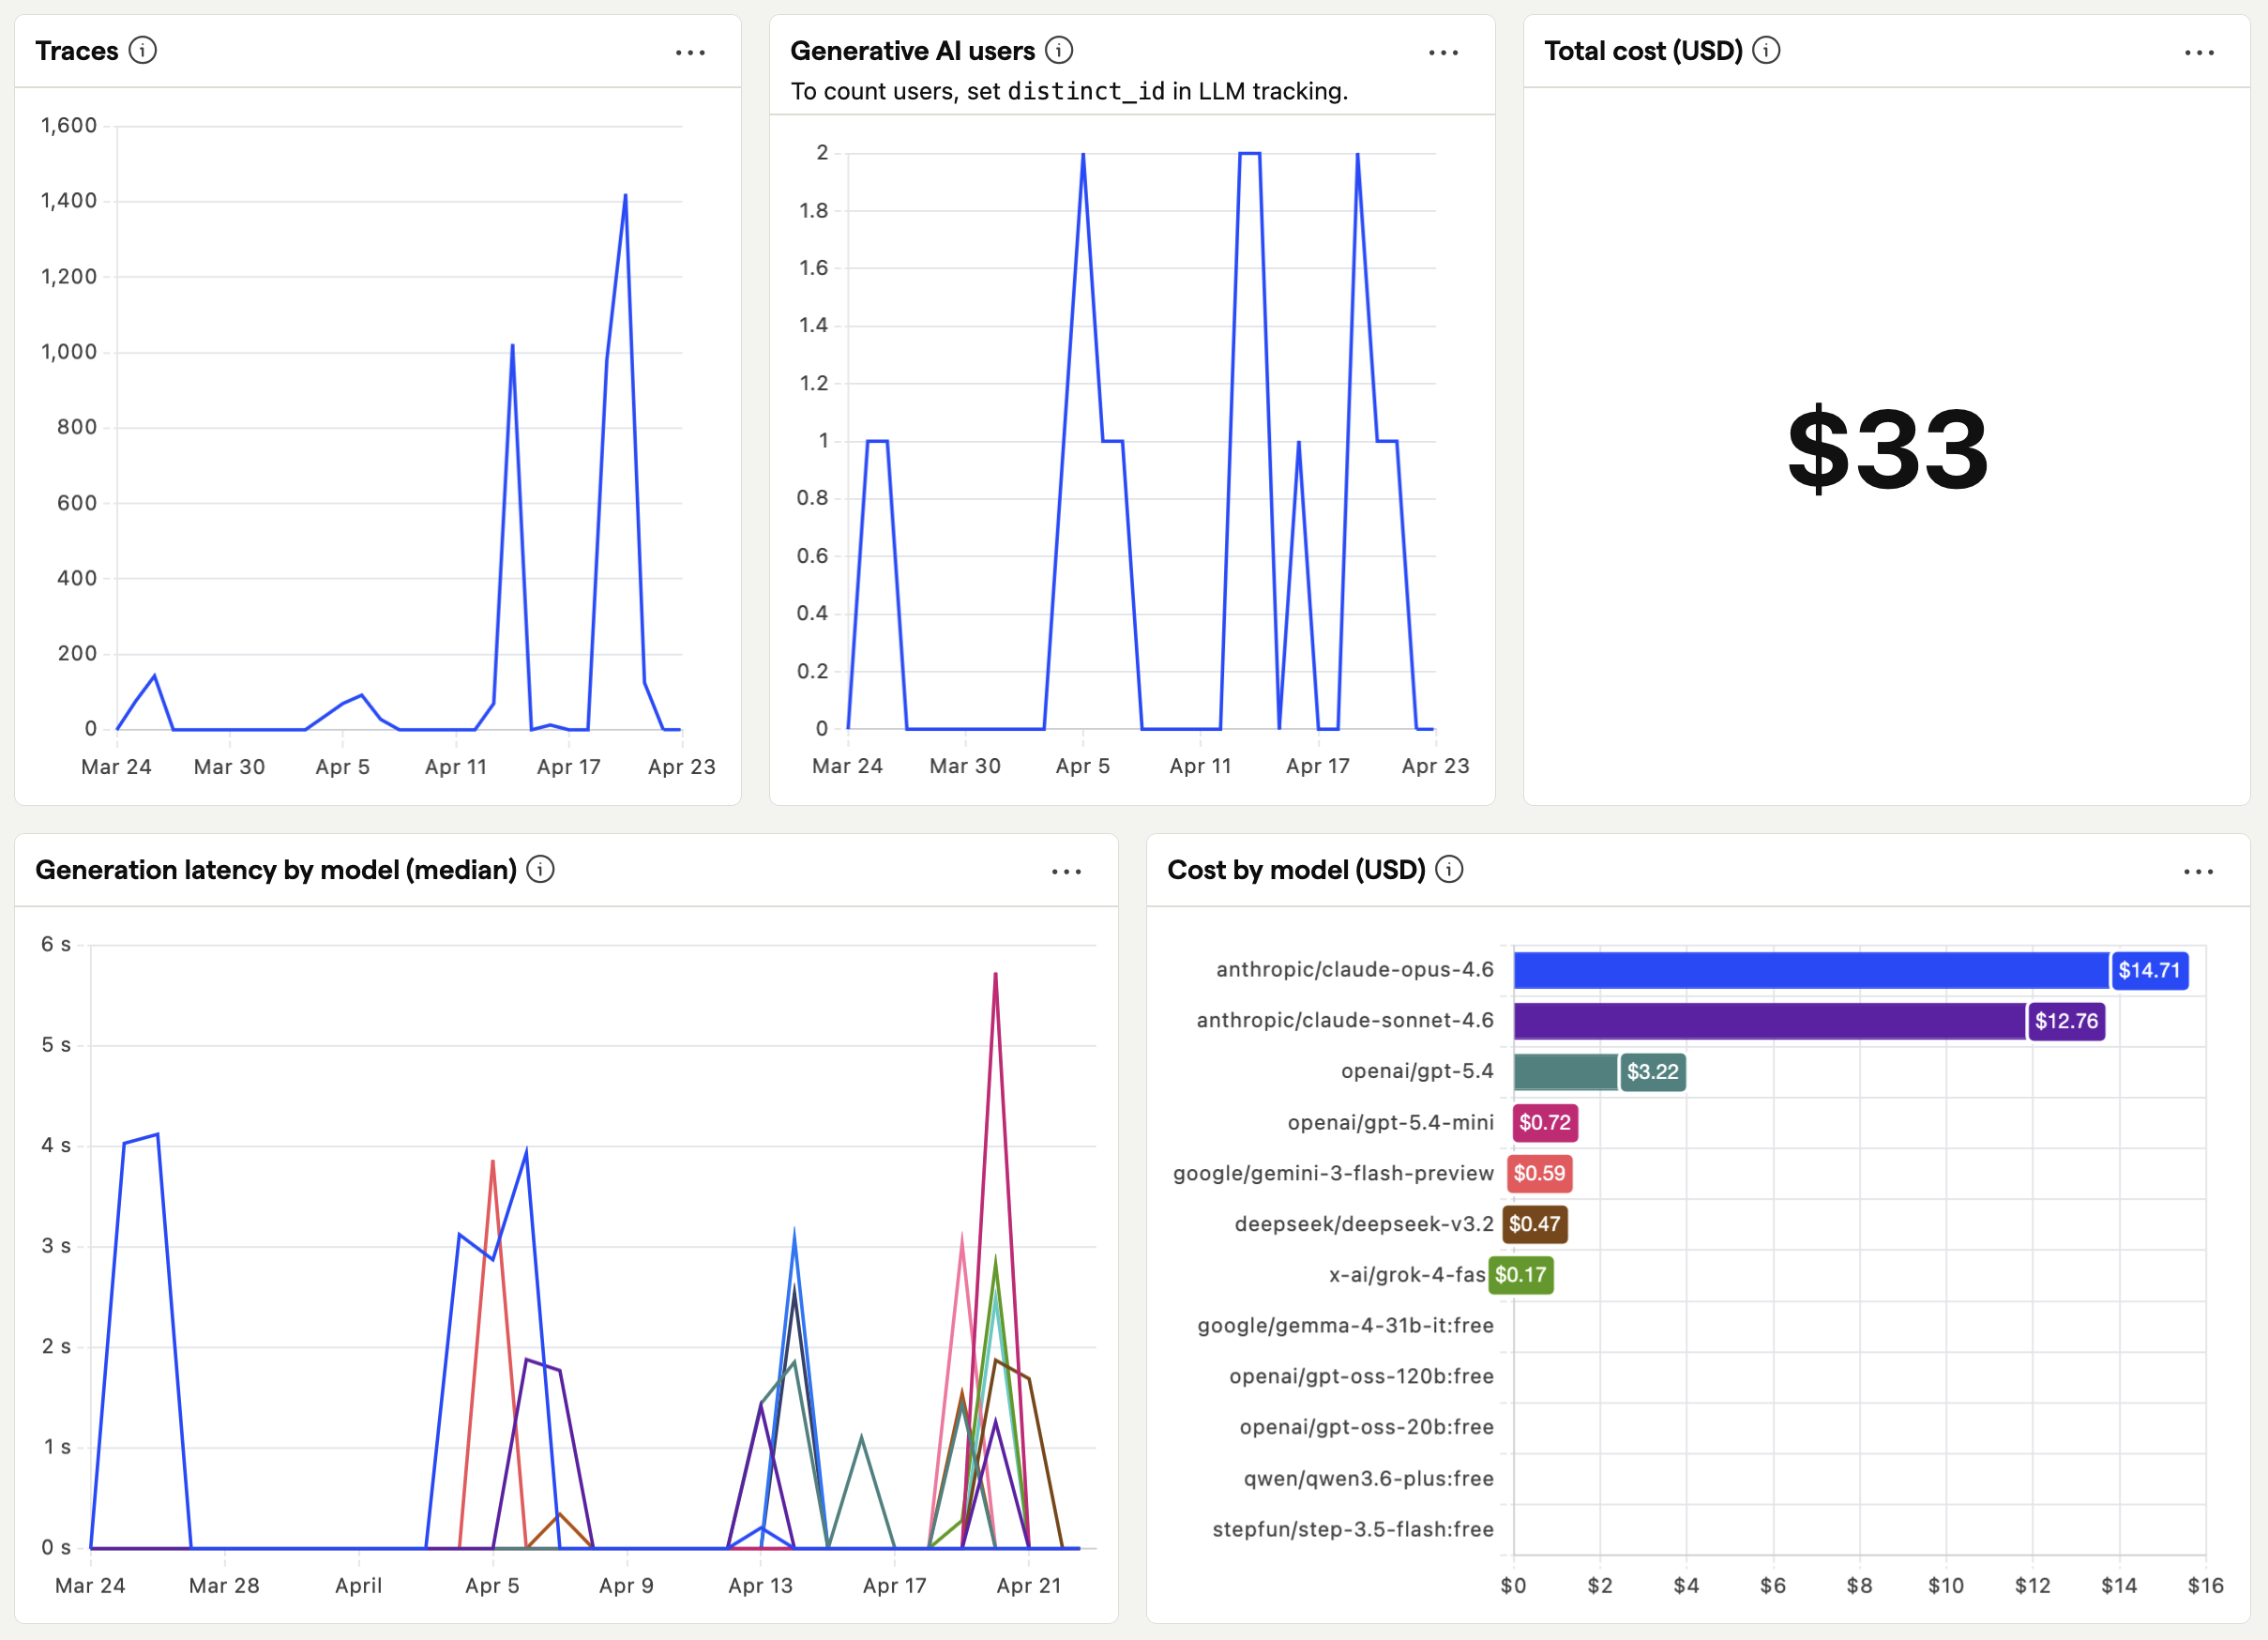
\includegraphics[width=\linewidth]{figures/posthog-dashboard.png}
    \caption{Aggregate analytics drive infrastructure and model-selection decisions.}
    \label{fig:posthog-dashboard}
\end{figure}

\begin{figure}
    \centering
    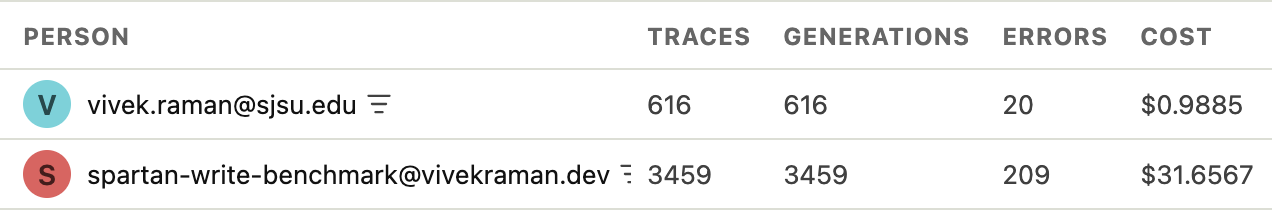
\includegraphics[width=0.8\linewidth]{figures/posthog-userwise.png}
    \caption{Per-user tracking reveals consumption patterns and usage anomalies.}
    \label{fig:posthog-userwise}
\end{figure}

\subsubsection{Safety \& ethical constraints}

The agent is designed with built-in safety mechanisms.

\begin{itemize}
    \item All file operations validate paths at the tooling level to prevent escaping the project directory.
    \item The prompt instructs the agent not to add unsolicited content.
    \item Compilation errors trigger error feedback rather than silent failures.
\end{itemize}
These constraints ensure the agent acts as a trusted scribe rather than an autonomous modifier.

\subsection{\LaTeX\ compilation}

The \LaTeX\ compilation subsystem is implemented as a sidecar component \cite{tauri_sidecar}.
The system leverages the Tectonic typesetting engine as its core compilation backend \cite{tectonic}.

Client requests containing the target project directory invoke the Tectonic compiler via subprocess execution with configurable parameters.
Process execution captures both standard output and error streams for diagnostic purposes.
The output PDF file path is displayed to the user upon successful generation.

Compilation can be initiated by either the user or the agent.
In the agent's case, the compilation status and error message are used to iteratively debug and fix the document.

\subsection{User guide}

The user guide is a lightweight static website consisting of instructions and references for users to get started with using Spartan Write.
It contains step-by-step guides on installation, usage, troubleshooting, and uninstallation of the program.
The website is built using MkDocs, a static site generator that converts markdown files into web pages \cite{mkdocs}.

\subsection{Benchmark}

The benchmark module is designed for testing the performance of various language models through the Spartan Write agent.
This is achieved using a reproducible test suite, consisting of a series of test documents and user requests along with different scoring metrics.
The benchmark module consists of four core components:
\begin{itemize}
    \item a CLI runner for orchestration;
    \item a scoring engine for metric evaluation;
    \item SQLite database storage for persistence;
    \item and a Streamlit dashboard for result visualization.
\end{itemize}

\subsubsection{Flow}

The benchmark execution follows a well-defined pipeline.
\begin{itemize}
    \item First, the dataset is loaded into the result directory and the database is initialized.
    \item For each test case, the tool prepares a workspace directory and sends the prompt to the agent server.
    \item After the chat completes, the scoring engine processes results to extract tool usage, duration, and token consumption metrics.
    \item These metrics are stored in the database.
    \item The dashboard then aggregates results from the database and renders interactive visualizations.
\end{itemize}

\subsubsection{Tests design}

The tests written as part of the benchmark are tabulated in Table \ref{tab:tests}.
They can be categorized as follows.

\begin{table}[htb]
\centering
\begin{tabularx}{\textwidth}{|l|X|}
\hline
\textbf{Test ID} & \textbf{Description} \\
\hline
000-empty-section & Create a new empty section with a specified name. \\
\hline
001-title-and-sections & Set document title and scaffold initial sections. \\
\hline
002-add-contents-to-section & Add multi-line content to an existing section. \\
\hline
003-remove-contents-from-section & Remove a specific line from a section. \\
\hline
004-large-unarranged-doc & Restructure and fix an unorganized document's file structure. \\
\hline
005-summarize-large-doc & Generate a concise summary of a large document. \\
\hline
006-large-new-section & Add a new section with specific detailed contents. \\
\hline
007-large-remove-contents & Remove a specific multi-line passage from a document. \\
\hline
008-large-search-fuzzy & Locate and pinpoint all discussions of a semantic topic. \\
\hline
009-large-remove-fuzzy & Remove all content discussing a particular semantic topic. \\
\hline
010-large-rearrange-sections & Swap the positions of two major sections. \\
\hline
011-large-rearrange-subsections & Swap major sections while preserving subsection hierarchy. \\
\hline
012-fail-to-generate-content & Attempt to generate content to test the agent's resilience against doing so. \\
\hline
013-large-add-image & Insert an attached diagram at a specified location in the document. \\
\hline
014-large-broken-explicit-fix & Diagnose and repair a broken LaTeX document via explicit instruction. \\
\hline
015-large-broken-implicit-fix & Repair a broken document through implicit problem inference. \\
\hline
016-large-parse-image & Interpret and describe the contents of an attached image. \\
\hline
\end{tabularx}
\caption{Benchmark test suite}
\label{tab:tests}
\end{table}

\begin{enumerate}
\item \textbf{Document structure manipulation} \\ 
    Tests 000, 001, 002, 003, 004, 006, 010, and 011 validate the core ability to create, modify, and reorganize LaTeX document structure.
    Each test assesses whether the LLM can correctly parse and modify the document hierarchy, including creating sections, adding and removing content, and reordering structural elements.
    Failures in this category would indicate difficulty understanding parent-child relationships in \LaTeX\ or an inability to preserve document integrity while making modifications. 
    These tests form the foundation of the benchmark, ensuring basic document operations function reliably.
\item \textbf{Search and targeted deletion} \\ 
    Tests 007, 008, and 009 evaluate the LLM's ability to find and remove content in large documents based on both exact and fuzzy matching criteria.
    These tests validate search accuracy across different scenarios: exact string matching for precise deletions, and semantic fuzzy matching for content-aware removal across multiple similar passages.
    Failures in this category would reveal whether the model struggles with context-aware removal, incorrectly handles ambiguous references, or lacks the precision needed for targeted edits.
\item \textbf{Document understanding and synthesis} \\
    Tests 005 and 012 measure the LLM's comprehension of full documents and its ability to generate summaries or new content in context. Test 005 requires distilling a large document into a coherent summary, while test 012 requires generating new content that matches the document's scope and tone. Failures would suggest poor long-context comprehension or an inability to maintain consistency with existing document material.
\item \textbf{Error recovery and problem diagnosis} \\ 
    Tests 014 and 015 assess the LLM's ability to recognize and fix broken \LaTeX\ documents with varying degrees of explicitness.
    Test 014 provides an explicit ''Fix the document'' instruction, while test 015 uses an indirect instruction to infer the need for repairs.
    These tests measure diagnostic capability and responsiveness to both explicit and implicit problem-solving cues.
    Failures would indicate weak error detection, an inability to infer intent from context, or insufficient \LaTeX\ syntax knowledge.
\item \textbf{Multimodal integration} \\ 
    Tests 013 and 016 evaluate the LLM's ability to work with visual attachments and integrate them into \LaTeX\ documents.
    Test 013 requires inserting an image reference in the appropriate location within the document, while test 016 requires visual comprehension and description of image contents.
    Failures in this category would reveal struggles with image understanding, file reference generation, or determining appropriate placement in the document structure.
\end{enumerate}

\subsubsection{Scoring metrics}

The scoring engine evaluates three primary metrics across each benchmark run.
\textbf{Tool use} aggregates tool calls by name and counts invocations per tool type, providing insight into which capabilities the LLM utilized.
\textbf{Chat duration} calculates the time taken for the agent to complete the task. This is primarily used to identify degradation in performance due to LLM updates or provider outages.
\textbf{Token usage} sums input tokens, output tokens, and reasoning tokens across all AI messages, tracking resource consumption.

\subsubsection{Dashboard}

The dashboard provides a Streamlit-based interactive web interface \cite{streamlit} that loads all results from the benchmark database and organizes them by model and test job.
Users can filter results by selected models, execution status (pending/complete/failed), error presence, and keyword search across job IDs and test summaries, as seen in Figure \ref{fig:bench-dashboard}.
The interface renders Plotly charts \cite{plotly} comparing scores across models and showing score distributions for deeper analysis.
Dashboard views also display run-level details including error messages, chat results, and individual run metrics.
Results are grouped by test job ID, with derived fields showing the latest status and scores from the most recent run of each job.

\begin{figure}[htb]
    \centering
    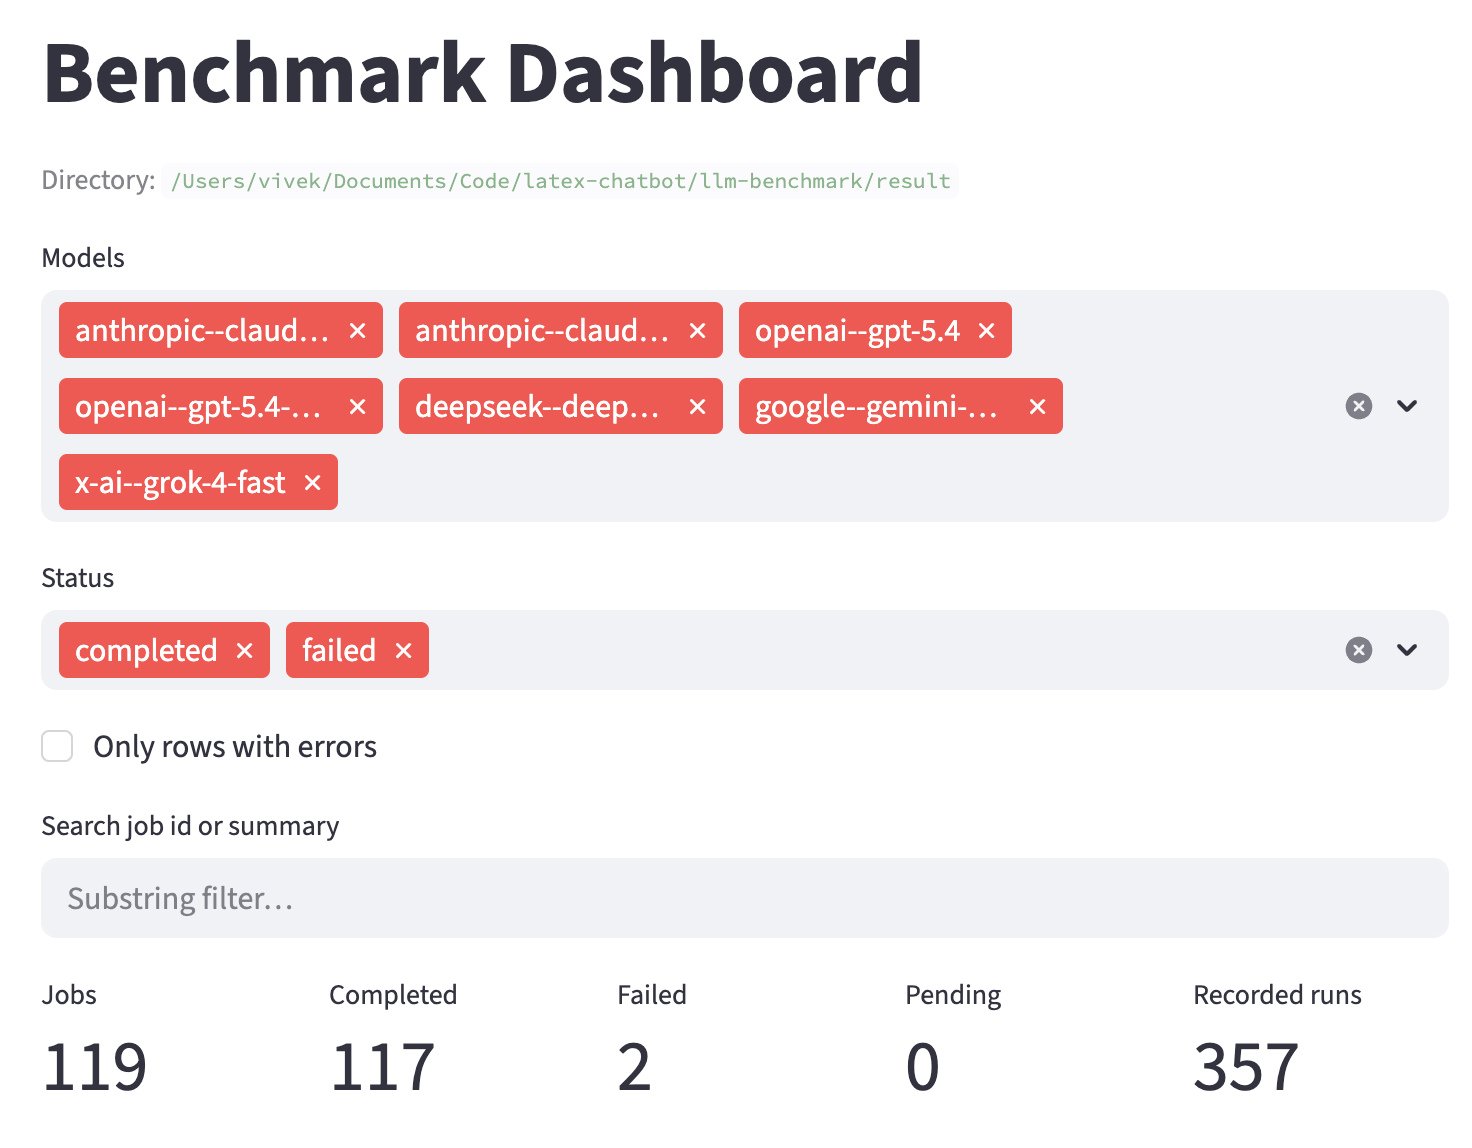
\includegraphics[width=0.67\linewidth]{figures/bench-dashboard.png}
    \caption{Filtering capabilities enable task-specific performance comparison.}
    \label{fig:bench-dashboard}
\end{figure}
